\documentclass[11pt,oneside]{article}
\usepackage[T1]{fontenc}
\usepackage[utf8]{inputenc}
% \usepackage{lmodern}
%\usepackage[adobe-utopia,uppercase=upright,greeklowercase=upright]{mathdesign}
\usepackage[adobe-utopia]{mathdesign}
%\usepackage{minionpro}
% \usepackage{pifont}
% \usepackage{amssymb}
\usepackage{amsmath}
\usepackage[francais]{babel}
% \usepackage[francais]{varioref}
\usepackage[dvips]{graphicx}

\usepackage{framed}
\usepackage[normalem]{ulem}
\usepackage{fancyhdr}
\usepackage{titlesec}
\usepackage{vmargin}
\usepackage{longtable}

\usepackage{ifthen}


%\usepackage{epsfig}
\usepackage{subfig}

\usepackage{multirow}
\usepackage{multicol} % Portions de texte en colonnes
\usepackage{flafter}%floatants après la référence



\usepackage{color}
\usepackage{colortbl}


\definecolor{gris25}{gray}{0.75}
\definecolor{bleu}{RGB}{18,33,98}
\definecolor{bleuf}{RGB}{42,94,171}
\definecolor{bleuc}{RGB}{231,239,247}
\definecolor{rougef}{RGB}{185,18,27}
\definecolor{rougec}{RGB}{255,230,231}
\definecolor{vertf}{RGB}{103,126,82}
\definecolor{vertc}{RGB}{220,255,191}
\definecolor{violetf}{RGB}{112,48,160}
\definecolor{violetc}{RGB}{230,224,236}

\newenvironment{sci}[1][\hsize]%
{%
    \def\FrameCommand%
    {%
%\rotatebox{90}{\textit{\textsf{Scilab}}\includegraphics[height=.8cm]{png/logo_scilab}} 
\rotatebox{90}{\includegraphics[height=.6cm]{png/logo_scilab}} 
        {\color{violetf}\vrule width 3pt}%
        \hspace{0pt}%must no space.
        \fboxsep=\FrameSep\colorbox{violetc}%
    }%
    \MakeFramed{\hsize #1 \advance\hsize-\width\FrameRestore}%
}%
{\endMakeFramed}%

\newenvironment{pseudo}[1][\hsize]%
{%
    \def\FrameCommand%
    {%
\rotatebox{90}{\textit{\textsf{Pseudo Code}}} 
        {\color{violetf}\vrule width 3pt}%
        \hspace{0pt}%must no space.
        \fboxsep=\FrameSep\colorbox{violetc}%
    }%
    \MakeFramed{\hsize #1 \advance\hsize-\width\FrameRestore}%
}%
{\endMakeFramed}%

\newenvironment{py}[1][\hsize]%
{%
    \def\FrameCommand%
    {%
%\rotatebox{90}{\textit{\textsf{Python}}} 
\rotatebox{90}{\includegraphics[height=.6cm]{png/logo_python}} 
        {\color{violetf}\vrule width 3pt}%
        \hspace{0pt}%must no space.
        \fboxsep=\FrameSep\colorbox{violetc}%
    }%
    \MakeFramed{\hsize #1 \advance\hsize-\width\FrameRestore}%
}%
{\endMakeFramed}%


\newenvironment{corrige}[1][\hsize]%
{%
    \def\FrameCommand
    {%
\rotatebox{90}{\textit{\textsf{Correction}}} 
        {\color{violetf}\vrule width 3pt}%
        \hspace{0pt}%must no space.
        \fboxsep=\FrameSep\colorbox{violetc}%
    }%
    \MakeFramed{\hsize#1\advance\hsize-\width\FrameRestore}%
}%
{\endMakeFramed}%



\newenvironment{rem}[1][\hsize]%
{%
    \def\FrameCommand
    {%
\rotatebox{90}{\textit{\textsf{Remarque}}} 
        {\color{bleuf}\vrule width 3pt}%
        \hspace{0pt}%must no space.
        \fboxsep=\FrameSep\colorbox{bleuc}%
    }%
    \MakeFramed{\hsize#1\advance\hsize-\width\FrameRestore}%
}%
{\endMakeFramed}%


\newenvironment{savoir}[1][\hsize]%
{%
    \def\FrameCommand
    {%
\rotatebox{90}{\textit{\textsf{Savoir}}} 
        {\color{bleuf}\vrule width 3pt}%
        \hspace{0pt}%must no space.
        \fboxsep=\FrameSep\colorbox{bleuc}%
    }%
    \MakeFramed{\hsize#1\advance\hsize-\width\FrameRestore}%
}%
{\endMakeFramed}%

\newenvironment{prob}[1][\hsize]%
{%
    \def\FrameCommand%
    {%
\rotatebox{90}{\textit{\textsf{ Problématique}}} 
        {\color{rougef}\vrule width 3pt}%
        \hspace{0pt}%must no space.
        \fboxsep=\FrameSep\colorbox{rougec}%
    }%
    \MakeFramed{\hsize#1\advance\hsize-\width\FrameRestore}%
}%
{\endMakeFramed}%

\newenvironment{obj}[1][\hsize]%
{%
    \def\FrameCommand%
    {%
\rotatebox{90}{\textit{\textsf{ $\;$}}} 
        {\color{rougef}\vrule width 3pt}%
        \hspace{0pt}%must no space.
        \fboxsep=\FrameSep\colorbox{rougec}%
    }%
    \MakeFramed{\hsize#1\advance\hsize-\width\FrameRestore}%
}%
{\endMakeFramed}%

\newenvironment{defi}[1][\hsize]%
{%
    \def\FrameCommand%
    {%
\rotatebox{90}{\textit{\textsf{Définition\\}}} 
        {\color{bleuf}\vrule width 3pt}%
        \hspace{0pt}%must no space.
        \fboxsep=\FrameSep\colorbox{bleuc}%
    }%
    \MakeFramed{\hsize#1\advance\hsize-\width\FrameRestore}%
}%
{\endMakeFramed}%


\newenvironment{demo}[1][\hsize]%
{%
    \def\FrameCommand%
    {%
\rotatebox{90}{\textit{\textsf{Démonstration\\}}} 
        {\color{bleuf}\vrule width 3pt}%
        \hspace{0pt}%must no space.
        \fboxsep=\FrameSep\colorbox{bleuc}%
    }%
    \MakeFramed{\hsize#1\advance\hsize-\width\FrameRestore}%
}%
{\endMakeFramed}%


\newenvironment{hypo}[1][\hsize]%
{%
    \def\FrameCommand%
    {%
\rotatebox{90}{\textit{\textsf{Hypothèse\\}}} 
        {\color{bleuf}\vrule width 3pt}%
        \hspace{0pt}%must no space.
        \fboxsep=\FrameSep\colorbox{bleuc}%
    }%
    \MakeFramed{\hsize#1\advance\hsize-\width\FrameRestore}%
}%
{\endMakeFramed}%


\newenvironment{prop}[1][\hsize]%
{%
    \def\FrameCommand%
    {%
\rotatebox{90}{\textit{\textsf{Propriété\\}}} 
        {\color{bleuf}\vrule width 3pt}%
        \hspace{0pt}%must no space.
        \fboxsep=\FrameSep\colorbox{bleuc}%
    }%
    \MakeFramed{\hsize#1\advance\hsize-\width\FrameRestore}%
}%
{\endMakeFramed}%

\newenvironment{props}[1][\hsize]%
{%
    \def\FrameCommand%
    {%
\rotatebox{90}{\textit{\textsf{Propriétés\\}}} 
        {\color{bleuf}\vrule width 3pt}%
        \hspace{0pt}%must no space.
        \fboxsep=\FrameSep\colorbox{bleuc}%
    }%
    \MakeFramed{\hsize#1\advance\hsize-\width\FrameRestore}%
}%
{\endMakeFramed}%

\newenvironment{exemple}[1][\hsize]%
{%
    \def\FrameCommand%
    {%
\rotatebox{90}{\textit{\textsf{Exemple\\}}} 
        {\color{vertf}\vrule width 3pt}%
        \hspace{0pt}%must no space.
        \fboxsep=\FrameSep\colorbox{vertc}%
    }%
    \MakeFramed{\hsize#1\advance\hsize-\width\FrameRestore}%
}%
{\endMakeFramed}%

\newenvironment{resultat}[1][\hsize]%
{%
    \def\FrameCommand%
    {%
\rotatebox{90}{\textit{\textsf{Résultat\\}}} 
        {\color{rougef}\vrule width 3pt}%
        \hspace{0pt}%must no space.
        \fboxsep=\FrameSep\colorbox{rougec}%
    }%
    \MakeFramed{\hsize#1\advance\hsize-\width\FrameRestore}%
}%
{\endMakeFramed}%

\newenvironment{methode}[1][\hsize]%
{%
    \def\FrameCommand%
    {%
\rotatebox{90}{\textit{\textsf{Méthode\\}}} 
        {\color{rougef}\vrule width 3pt}%
        \hspace{0pt}%must no space.
        \fboxsep=\FrameSep\colorbox{rougec}%
    }%
    \MakeFramed{\hsize#1\advance\hsize-\width\FrameRestore}%
}%
{\endMakeFramed}%

\newenvironment{theo}[1][\hsize]%
{%
    \def\FrameCommand%
    {%
\rotatebox{90}{\textit{\textsf{Théorème\\}}} 
        {\color{rougef}\vrule width 3pt}%
        \hspace{0pt}%must no space.
        \fboxsep=\FrameSep\colorbox{rougec}%
    }%
    \MakeFramed{\hsize#1\advance\hsize-\width\FrameRestore}%
}%
{\endMakeFramed}%

\newenvironment{warn}[1][\hsize]%
{%
    \def\FrameCommand%
    {%
\rotatebox{90}{\textit{\textsf{Attention\\}}} 
        {\color{rougef}\vrule width 3pt}%
        \hspace{0pt}%must no space.
        \fboxsep=\FrameSep\colorbox{rougec}%
    }%
    \MakeFramed{\hsize#1\advance\hsize-\width\FrameRestore}%
}%
{\endMakeFramed}%

% \usepackage{pstricks}
%\usepackage{minitoc}
% \setcounter{minitocdepth}{4}

\setcounter{tocdepth}{2}

% \mtcselectlanguage{french} 

%\usepackage{draftcopy}% "Brouillon"
% \usepackage{floatflt}
\usepackage{psfrag}
%\usepackage{listings} % Permet d'insérer du code de programmation
\renewcommand{\baselinestretch}{1.2}

% Changer la numérotation des figures :
% ------------------------------------
% \makeatletter
% \renewcommand{\thefigure}{\ifnum \c@section>\z@ \thesection.\fi
%  \@arabic\c@figure}
% \@addtoreset{figure}{section}
% \makeatother
 


%%%%%%%%%%%%
% Définition des vecteurs %
%%%%%%%%%%%%
 \newcommand{\vect}[1]{\overrightarrow{#1}}

%%%%%%%%%%%%
% Définition des torseusr %
%%%%%%%%%%%%

 \newcommand{\torseur}[1]{%
\left\{{#1}\right\}
}

\newcommand{\torseurcin}[3]{%
\left\{\mathcal{#1} \left(#2/#3 \right) \right\}
}

\newcommand{\torseurstat}[3]{%
\left\{\mathcal{#1} \left(#2\rightarrow #3 \right) \right\}
}

 \newcommand{\torseurc}[8]{%
%\left\{#1 \right\}=
\left\{
{#1}
\right\}
 = 
\left\{%
\begin{array}{cc}%
{#2} & {#5}\\%
{#3} & {#6}\\%
{#4} & {#7}\\%
\end{array}%
\right\}_{#8}%
}

 \newcommand{\torseurcol}[7]{
\left\{%
\begin{array}{cc}%
{#1} & {#4}\\%
{#2} & {#5}\\%
{#3} & {#6}\\%
\end{array}%
\right\}_{#7}%
}

 \newcommand{\torseurl}[3]{%
%\left\{\mathcal{#1}\right\}_{#2}=%
\left\{%
\begin{array}{l}%
{#1} \\%
{#2} %
\end{array}%
\right\}_{#3}%
}

 \newcommand{\vectv}[3]{%
\vect{V\left( {#1} \in {#2}/{#3}\right)}
}


\newcommand{\vectf}[2]{%
\vect{R\left( {#1} \rightarrow {#2}\right)}
}

\newcommand{\vectm}[3]{%
\vect{\mathcal{M}\left( {#1}, {#2} \rightarrow {#3}\right)}
}


 \newcommand{\vectg}[3]{%
\vect{\Gamma \left( {#1} \in {#2}/{#3}\right)}
}

 \newcommand{\vecto}[2]{%
\vect{\Omega\left( {#1}/{#2}\right)}
}
% }$$\left\{\mathcal{#1} \right\}_{#2} =%
% \left\{%
% \begin{array}{c}%
%  #3 \\%
%  #4 %
% \end{array}%
% \right\}_{#5}}

%  ------------------------------------------
% | Modification du formatage des sections : | 
%  ------------------------------------------

% Grands titres :
% ---------------

\newcommand{\titre}[1]{%
\begin{center}
      \bigskip
      \rule{\textwidth}{1pt}
      \par\vspace{0.1cm}
      
      \textbf{\large #1}
      \par\rule{\textwidth}{1pt}
    \end{center}
    \bigskip
  }

% Supprime le numéro du chapitre dans la numérotation des sections:
% -----------------------------------------------------------------
\makeatletter
\renewcommand{\thesection}{\@arabic\c@section}
\makeatother


% \titleformat{\chapter}[display]
% {\normalfont\Large\filcenter}
% {}
% {1pc}
% {\titlerule[1pt]
%   \vspace{1pc}%
%   \Huge}[\vspace{1ex}%
% \titlerule]


%%%% Chapitres Comme PY Pechard %%%%%%%%%
% numéro du chapitre
\DeclareFixedFont{\chapnumfont}{OT1}{phv}{b}{n}{80pt}
% pour le mot « Chapitre »
\DeclareFixedFont{\chapchapfont}{OT1}{phv}{m}{it}{40pt}
% pour le titre
\DeclareFixedFont{\chaptitfont}{T1}{phv}{b}{n}{25pt}

\definecolor{gris}{gray}{0.75}
\titleformat{\chapter}[display]%
	{\sffamily}%
	{\filleft\chapchapfont\color{gris}\chaptertitlename\
	\\
	\vspace{12pt}
	\chapnumfont\thechapter}%
	{16pt}%
	{\filleft\chaptitfont}%
	[\vspace{6pt}\titlerule\titlerule\titlerule]

%%%%  Fin Chapitres Comme PY Pechard %%%%%%%%%


% Section, subsection, subsubsection sans serifs :
% % ----------------------------------------------

% \makeatletter
% \renewcommand{\section}{\@startsection{section}{0}{0mm}%
% {\baselineskip}{.3\baselineskip}%
% {\normalfont\sffamily\Large\textbf}}%
% \makeatother

\makeatletter
\renewcommand{\@seccntformat}[1]{{\textcolor{bleu}{\csname
the#1\endcsname}\hspace{0.5em}}}
\makeatother

\makeatletter
\renewcommand{\section}{\@startsection{section}{1}{\z@}%
                       {-4ex \@plus -1ex \@minus -.4ex}%
                       {1ex \@plus.2ex }%
                       {\normalfont\Large\sffamily\bfseries}}%
\makeatother
 
\makeatletter
\renewcommand{\subsection}{\@startsection {subsection}{2}{\z@}
                          {-3ex \@plus -0.1ex \@minus -.4ex}%
                          {0.5ex \@plus.2ex }%
                          {\normalfont\large\sffamily\bfseries}}
\makeatother
 
\makeatletter
\renewcommand{\subsubsection}{\@startsection {subsubsection}{3}{\z@}
                          {-2ex \@plus -0.1ex \@minus -.2ex}%
                          {0.2ex \@plus.2ex }%
                          {\normalfont\large\sffamily\bfseries}}
\makeatother
 
\makeatletter             
\renewcommand{\paragraph}{\@startsection{paragraph}{4}{\z@}%
                                    {-2ex \@plus-.2ex \@minus .2ex}%
                                    {0.1ex}%               
{\normalfont\sffamily\bfseries}}
\makeatother
 

\makeatletter             
\renewcommand{\subparagraph}{\@startsection{subparagraph}{5}{\z@}%
                                    {-2ex \@plus-.2ex \@minus .2ex}%
                                    {0.1ex}%               
{\normalfont\bfseries Question }}
\makeatother

\renewcommand{\thesubparagraph}{\arabic{subparagraph}} 
%
\makeatletter
%\renewcommand{\subparagraph}{\@startsection{subparagraph}{5}{\z@}%
%                                       {-2ex \@plus-.1ex \@minus .2ex}%
%                                       {0.1ex}%
%				    {\normalfont\normalsize\sffamily\bfseries}}
%\makeatletter
% \makeatletter
% \renewcommand{\subsection}{\@startsection{subsection}{1}{2mm}%
% {\baselineskip}{.3\baselineskip}%
% {\normalfont\sffamily\large\textbf}}%
% \makeatother
% 
% \makeatletter
% \renewcommand{\subsubsection}{\@startsection{subsubsection}{2}{4mm}%
% {\baselineskip}{.15\baselineskip}%
% {\normalfont\sffamily\large\textbf}}%
% \makeatother
% 
% \makeatletter
% \renewcommand{\paragraph}{\@startsection{paragraph}{3}{6mm}%
% {\baselineskip}{.15\baselineskip}%
% {\normalfont\sffamily\large\textbf}}%
% \makeatother
 
\setcounter{secnumdepth}{5}


%  --------
% | Marges |
%  --------


% \setmarginsrb{2.5cm}{1.5cm}{2.5cm}{2cm}{1cm}{1cm}{1cm}{1cm}
\setmarginsrb{1.5cm}{1cm}{1cm}{1.5cm}{1cm}{1cm}{1cm}{1cm}

% Changer les marges localement :
% -----------------------------
\newenvironment{changemargin}[2]{\begin{list}{}{%
\setlength{\topsep}{0pt}%
\setlength{\leftmargin}{0pt}%
\setlength{\rightmargin}{0pt}%
\setlength{\listparindent}{\parindent}%
\setlength{\itemindent}{\parindent}%
\setlength{\parsep}{0pt plus 1pt}%
\addtolength{\leftmargin}{#1}%
\addtolength{\rightmargin}{#2}%
}\item }{\end{list}}



\usepackage{pst-solides3d}
\usepackage{titletoc}
\titlecontents{chapter}[+3pc]
  {\addvspace{10pt}\sffamily\bfseries}
{\contentslabel[{\pscirclebox[fillstyle=solid,fillcolor=gray!25,
linecolor=gray!25,framesep=4pt]{\textcolor{white}{\thecontentslabel}}}]{2.5pc}}
  {}
  {\dotfill \normalfont\thecontentspage\ }

\titlecontents{section}[3pc]
  {\addvspace{2pt}\sffamily}
  {\contentslabel[\thecontentslabel]{1.8pc}}
  {}
  {\dotfill \normalfont\thecontentspage\ }

\titlecontents{subsection}[5pc]
  {\addvspace{2pt}\sffamily}
  {\contentslabel[\thecontentslabel]{1.8pc}}
  {}
  {\dotfill \normalfont\thecontentspage\ }

\titlecontents{subsubsection}[8pc]
  {\addvspace{2pt}\sffamily}
  {\contentslabel[\thecontentslabel]{3pc}}
  {}
  {\dotfill \normalfont\thecontentspage\ }
%{\;\titlerule\;\normalfont\thecontentspage\ }

\titlecontents{paragraph}[9pc]
  {\addvspace{2pt}\sffamily}
  {\contentslabel[\thecontentslabel]{3.5pc}}
  {}
  {\dotfill \normalfont\thecontentspage\ }




\usepackage[%
    pdftitle={SLCI -- Systèmes du second ordre -- TD},
    pdfauthor={Xavier Pessoles},
    colorlinks=true,
    linkcolor=blue,
    citecolor=magenta]{hyperref}



% \makeatletter \let\ps@plain\ps@empty \makeatother
%% DEBUT DU DOCUMENT
%% =================
\sloppy
\hyphenpenalty 10000

\newcommand{\Pointilles}[1][3]{%
\multido{}{#1}{\makebox[\linewidth]{\dotfill}\\[\parskip]
}}


\begin{document}


\newboolean{prof}
\setboolean{prof}{false}
%------------- En tetes et Pieds de Pages ------------
\pagestyle{fancy}
\renewcommand{\headrulewidth}{0pt}

\fancyhead{}
\fancyhead[L]{%
\noindent\noindent\begin{minipage}[c]{2.6cm}
%Lycée Rouvière PTSI

\includegraphics[width=2cm]{png/logo_ptsi.png}%
\end{minipage}
}

\fancyhead[C]{\rule{12cm}{.5pt}}

\fancyhead[R]{%
\begin{minipage}[c]{3cm}
\begin{flushright}
\footnotesize{\textit{\textsf{Sciences Industrielles\\ de l'Ingénieur}}}%
\end{flushright}
\end{minipage}
}

\renewcommand{\footrulewidth}{0.2pt}

\fancyfoot[C]{\footnotesize{\bfseries \thepage}}
\fancyfoot[L]{\footnotesize{2013 -- 2014} \\ X. \textsc{Pessoles}}
\ifthenelse{\boolean{prof}}{%
\fancyfoot[R]{\footnotesize{CI 2 : SLCI -- TD} \\ \footnotesize{Ch. 5 : Ordre 2 -- P}}
}{%
\fancyfoot[R]{\footnotesize{CI 2 : SLCI -- TD} \\ \footnotesize{Ch. 5 : Ordre 2 -- E}}
}


%\begin{center}
%\textit{Centre d'intérêt}
%\end{center}



\begin{center}
 \Large\textsc{CI 2 -- SLCI : Étude du comportement des Systèmes Linéaires Continus Invariants}
\end{center}

\begin{center}
 \large\textsc{Chapitre 5 -- Étude des systèmes fondamentaux du second ordre}
\end{center}

\begin{center}
\textsc{Travail dirigé -- Étude d'un laminoir} 
\end{center}

\begin{flushright}
\textit{D'après ressources de Jean-Pierre Pupier.} 
\end{flushright}


\vspace{.5cm}

\section{Introduction}
\subsection{Présentation de l'étude}

Une tôle est une plaque rectangulaire. Sa longueur est de l'ordre d'une centaine de mètres, sa largeur du mètre et son épaisseur du millimètre. Elle est conditionnée enroulée sur elle-même autour d'un fourreau (cf. figure 1). L'écrasement entre deux cylindres animés de mouvements de rotation antagonistes (cf. figure 2) permet de réduire l'épaisseur de la tôle. Cette opération s'appelle le laminage et la machine qui la réalise un laminoir. C'est un des plus importants procédés de mise en forme des métaux. Les produits issus du laminage sont utilisés en automobile, en électroménager, en emballage alimentaire...

\vspace{.25cm}

\noindent\begin{minipage}[c]{.48\linewidth}
\begin{center}
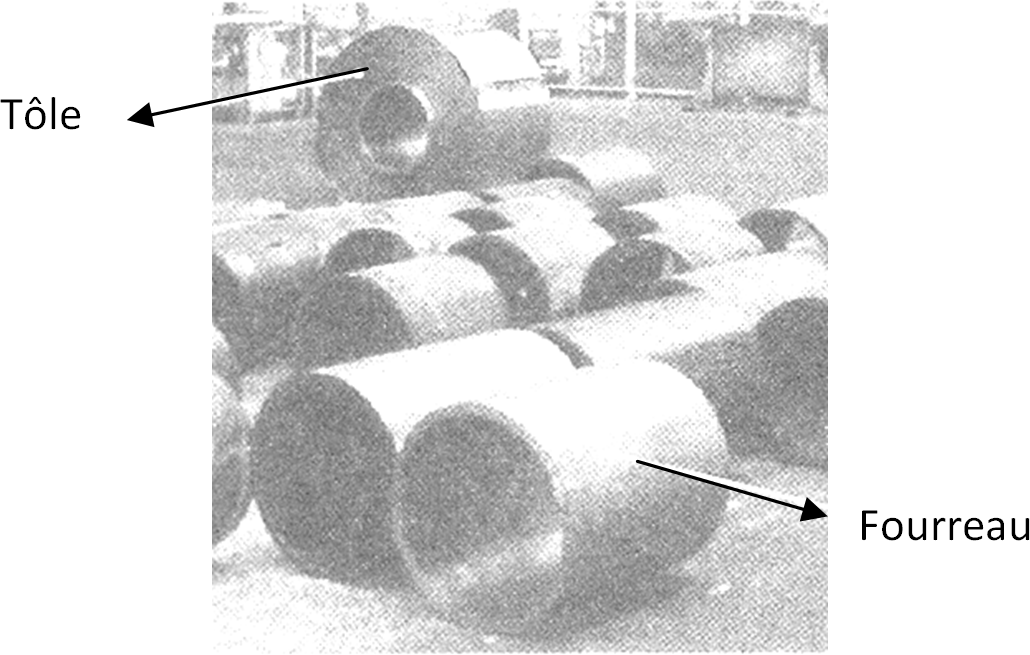
\includegraphics[width=.95\textwidth]{png/figure_01}

\textit{Figure 1 : Fourreaux et tôles conditionnées}
\end{center}
\end{minipage}\hfill
\begin{minipage}[c]{.48\linewidth}
\begin{center}
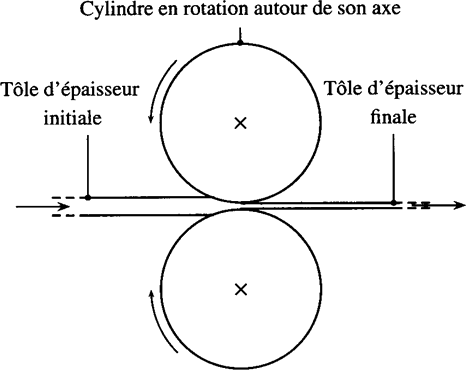
\includegraphics[width=.95\textwidth]{png/figure_02}

\textit{Figure 2 : Principe de base du laminage}
\end{center}
\end{minipage}\hfill


\subsection{Fonctionnement du laminoir Sendzimir}

\begin{center}
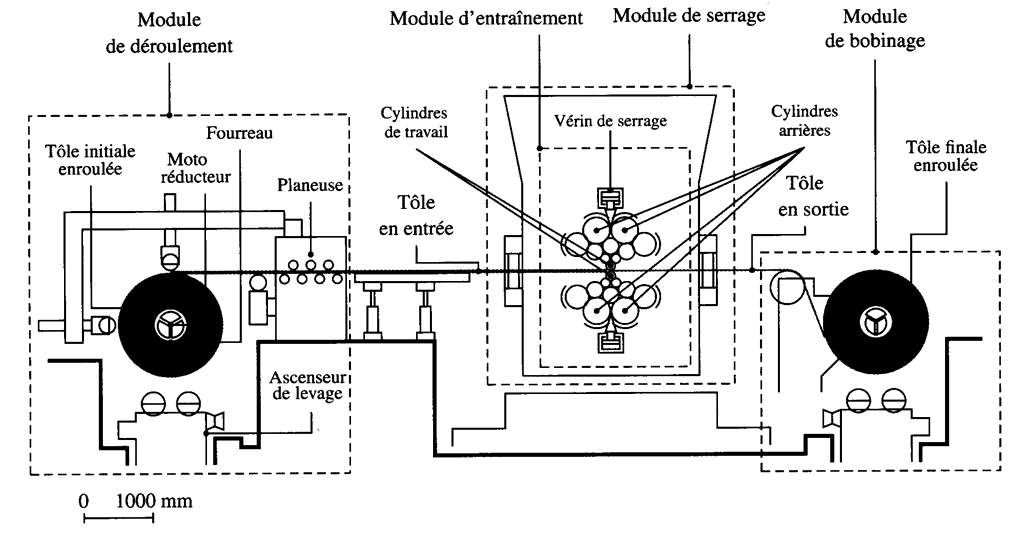
\includegraphics[width=.95\textwidth]{png/figure_03}

\textit{Figure 3 : Schéma d'un laminoir Sendzimir}
\end{center}

Le laminoir de type Sendzimir (cf. figure 3) permet de laminer les tôles métalliques. Plusieurs passes successives sont réalisées pour écraser progressivement la tôle. Pour la première passe, ce laminoir met en œuvre quatre modules :
\begin{itemize}
\item le module de déroulement: il a pour fonction de dérouler la tôle d'épaisseur initiale. Il est constitué principalement d'un moto-réducteur qui entraîne en rotation le fourreau, asservi de manière à assurer un effort de tension constant dans la tôle en entrée du laminoir. Ce module comporte également une planeuse qui redresse la tôle pour la rendre plane et un ascenseur de levage qui permet de charger la tôle.
\item le module d'entraînement de la tôle, appelé cage d'entraînement: il a pour fonction de faire avancer la tôle dans le laminoir. Il est constitué d'un mécanisme à plusieurs cylindres, entraînés en rotation par un moteur à courant continu, asservi en vitesse. Les cylindres de travail entraînent la tôle par adhérence.
\item le module de serrage: il a pour fonction de contrôler l'écrasement de la tôle. Il est constitué de plusieurs vérins hydrauliques asservis en position, appuyant sur les cylindres arrières.
\item le module de bobinage: il a pour fonction d'enrouler la tôle finale d'épaisseur réduite. Il est constitué d'un moto-réducteur, asservi de manière à assurer un effort de tension constant dans la tôle en sortie du laminoir.
\end{itemize}

\section{Étude de la fonction <<assurer l'entraînement de la tôle>>}

Pour assurer cette fonction il est nécessaire de réaliser le contrôle continu de la vitesse d'entraînement de la tôle dans le module d'entraînement du laminoir.

\subsection{Performance attendues}

Les performances attendues sont données par le tableau suivant.

\begin{center}
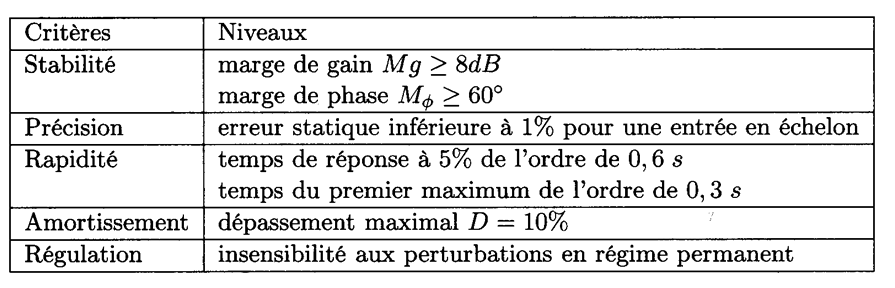
\includegraphics[width=.75\textwidth]{png/figure_04}
\end{center}

\subparagraph{}
\textit{Donner la définition d'un système stable. A quelle condition cela est-il vérifié ?}

\ifthenelse{\boolean{prof}}{
\begin{corrige}
\end{corrige}
}{}

\subparagraph{}
\textit{Donner la grandeur physique permettant de définir la rapidité d'un système. A l'aide d'une représentation graphique expliquer que la faculté d’un système à atteindre vite la grandeur physique souhaitée n’est pas forcément un gage de rapidité.}

\ifthenelse{\boolean{prof}}{
\begin{corrige}
\end{corrige}
}{}

\subparagraph{}
\textit{Donner la valeur de dépassement maximum qui ne pénalise pas le temps de réponse.}

\ifthenelse{\boolean{prof}}{
\begin{corrige}
\end{corrige}
}{}

\subparagraph{}
\textit{Expliquer la phrase <<insensibilité aux perturbations en régime permanent>>.}

\ifthenelse{\boolean{prof}}{
\begin{corrige}
\end{corrige}
}{}

\subsection{Chaîne fonctionnelle sans correcteur}

La chaîne fonctionnelle de l'asservissement en vitesse de l'entraînement de la tôle est schématisée par les schémas fonctionnels suivants. Le couple perturbateur $C_L$ modélise l'action d'entraînement de la tôle.

\begin{center}
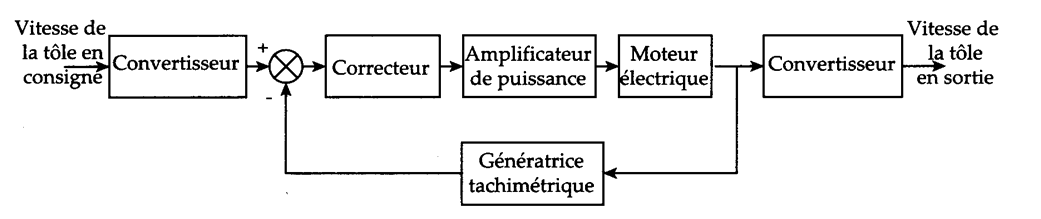
\includegraphics[width=.8\textwidth]{png/figure_05}

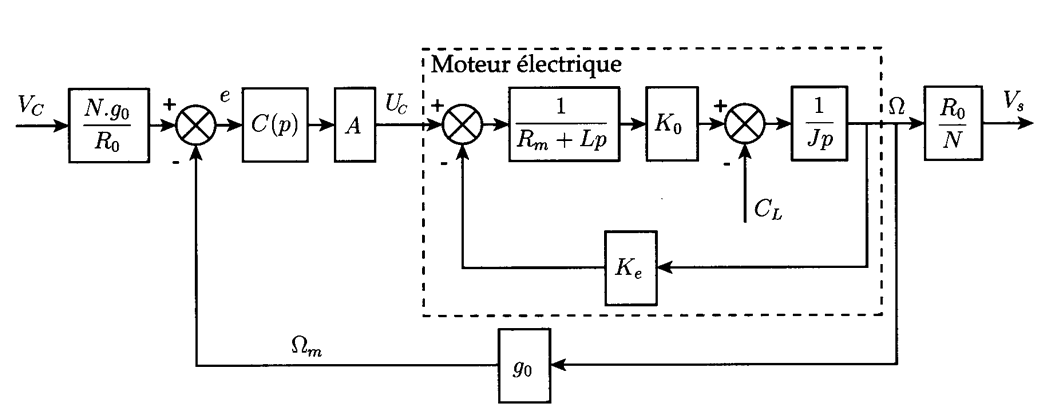
\includegraphics[width=.8\textwidth]{png/figure_06}

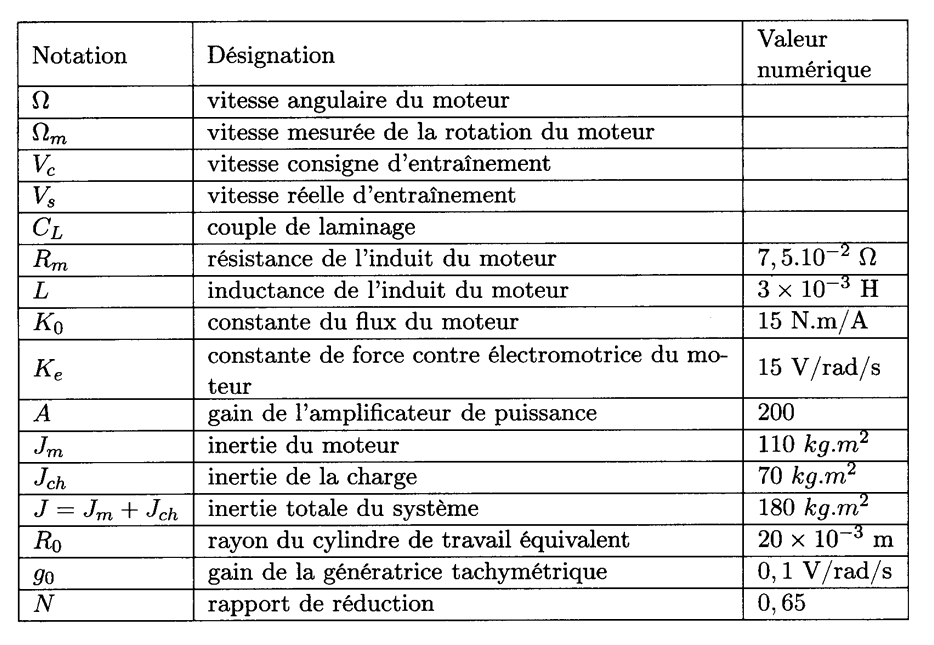
\includegraphics[width=.8\textwidth]{png/figure_07}
\end{center}

Pour le moment le système est sans correcteur c'est à dire que $C(p) = 1$.

On considère dans un premier temps que le couple de laminage $C_L$ est nul.

\subparagraph{}
\textit{Exprimer la fonction de transfert relative au moteur électrique $H_{mot}=\dfrac{\Omega(p)}{U_C(p)}$ et la mettre sous la forme $H_{mot}=\dfrac{K_{mot}}{a_1p^2+a_0 p +1}$ en précisant clairement l'expression littérale de $K_{mot}$, $a_0$ et $a_1$.}

\ifthenelse{\boolean{prof}}{
\begin{corrige}
\end{corrige}
}{}

\subparagraph{}
\textit{Calculer les valeurs numériques de $K_{mot}$, $a_0$ et $a_1$. Vous préciserez (évidemment) les unités.}

\ifthenelse{\boolean{prof}}{
\begin{corrige}
\end{corrige}
}{}


La fonction de transfert du moteur étant connue, le schéma fonctionnel du système étudié se met alors sous la forme suivante.

\begin{center}
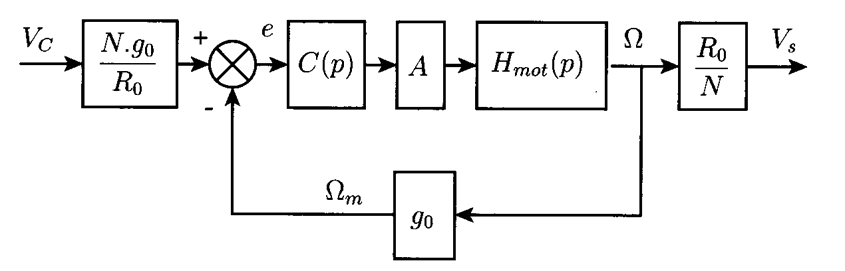
\includegraphics[width=.6\textwidth]{png/figure_08}
\end{center}

\subparagraph{}
\textit{Exprimez littéralement, en faisant intervenir $K_{mot}$, $a_0$ et $a_1$ la fonction de transfert en boucle ouverte $\dfrac{\Omega_m(p)}{e(p)}$.}

\ifthenelse{\boolean{prof}}{
\begin{corrige}
\end{corrige}
}{}

\subparagraph{}
\textit{Calculer la fonction de transfert en boucle fermée $\dfrac{V_S(p)}{V_C(p)}$.}

\ifthenelse{\boolean{prof}}{
\begin{corrige}
\end{corrige}
}{}

\subparagraph{}
\textit{Calculer les caractéristiques numériques de la fonction de transfert en boucle fermée :
\begin{itemize}
\item gain statique $K_{stat}$;
\item pulsation naturelle ou pulsation propre $\omega_0$;
\item amortissement $\xi$.
\end{itemize}
}

\ifthenelse{\boolean{prof}}{
\begin{corrige}
\end{corrige}
}{}


Les abaques donnés ci-dessous correspondent à un système du second ordre décrit par sa fonction de transfert en boucle fermée $F(p)=\dfrac{\omega_0^2}{p^2+2\xi\omega_0 p + \omega_0^2}$ .

\begin{center}
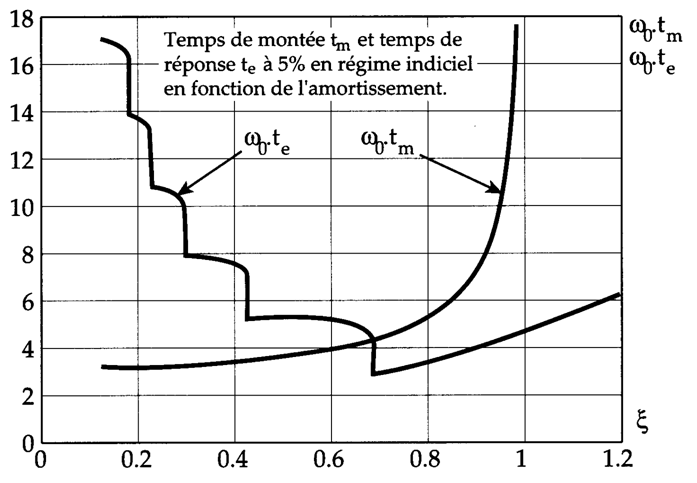
\includegraphics[width=.6\textwidth]{png/figure_09}

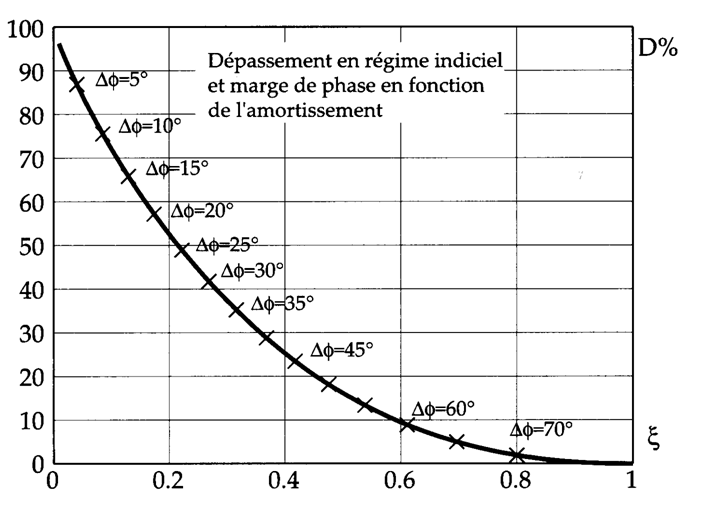
\includegraphics[width=.6\textwidth]{png/figure_10}
\end{center}

\subparagraph{}
\textit{A partir des abaques déterminer le premier dépassement en \% et le temps de réponse $t_e$  à 5\% à un échelon de consigne}

\ifthenelse{\boolean{prof}}{
\begin{corrige}
\end{corrige}
}{}

\subparagraph{}
\textit{Le temps du premier dépassement obtenu par les abaques est-il en cohérence avec la formule du cours : $T_m=\dfrac{\pi}{\omega_0\sqrt{1-\xi^2}}$ ?}

\ifthenelse{\boolean{prof}}{
\begin{corrige}
\end{corrige}
}{}

\subparagraph{}
\textit{Conclure quant à la pertinence d'un bouclage sans correction. Deux points sont à analyser : rapidité et amortissement.}

\ifthenelse{\boolean{prof}}{
\begin{corrige}
\end{corrige}
}{}

\subsection{Chaîne fonctionnelle avec correcteur proportionnel.}

Le correcteur a maintenant pour fonction de transfert $C(p) = K_C$.

\subparagraph{}
\textit{Calculer la fonction de transfert en boucle ouverte  $\dfrac{\Omega_m(p)}{e(p)}$ et en déduire la fonction de transfert en boucle fermée $\dfrac{V_S(p)}{V_C(p)}$.}

\ifthenelse{\boolean{prof}}{
\begin{corrige}
\end{corrige}
}{}

\subparagraph{}
\textit{Exprimer la valeur du gain $K_C$, notée $K_{C0}$, pour que le système en boucle fermée présente un dépassement de $D=10\%$. Calculer cette valeur. Faire l'application numérique. }

\ifthenelse{\boolean{prof}}{
\begin{corrige}
\end{corrige}
}{}
\end{document}
\subparagraph{}
\textit{}

\ifthenelse{\boolean{prof}}{
\begin{corrige}
\end{corrige}
}{}

\subparagraph{}
\textit{}

\ifthenelse{\boolean{prof}}{
\begin{corrige}
\end{corrige}
}{}

\subparagraph{}
\textit{}

\ifthenelse{\boolean{prof}}{
\begin{corrige}
\end{corrige}
}{}


